\documentclass[mathserif,notheorems,11pt]{beamer}
\usetheme{Warsaw}  %% Themenwahl
\usepackage[utf8]{inputenc}
\usefonttheme{serif}
\title{\textbf{University ranks}}
\author{\textsc{Back\'{e}} Julian, \textsc{Salzer} Tobias, \textsc{Singh} Ajayvir\\
Group 19}
\date{}
\usepackage{stmaryrd}
\usepackage{makecell}


%Julian
\begin{document}
\maketitle
\linespread{1.2}

%Julian
\begin{frame} 
\frametitle{Agenda / Questions}
\begin{itemize}
	\item How do university rankings change over time? 
	
	\item Which characteristics of universities contribute most to good rankings, or to large changes in the ranking position? 
	
	\item How do these characteristics correlate with characteristics of cities or countries in which the university is
	located? 
	
	\item Are there predictors for increases or decreases in the rankings?
\end{itemize}

\end{frame}

%Julian
\begin{frame} 
\frametitle{Workflow}


\begin{enumerate}
\item \textbf{Data acquisition and preprocessing}

\item \textbf{Data Exploration -- with results}

\item \textbf{Data Modelling -- with results}
\end{enumerate}
\end{frame}

%Ajay
\begin{frame} 
\frametitle{Data acquisition and loading}
\begin{itemize}
\item \textbf{Center for World University Rankings} (CWUR) $\rightarrow$ Main data source
\item \textbf{Academic Ranking of World Ranking Universities} $\rightarrow$ by ShanghaiRanking, contains rankings from 2005
\item \textbf{World University Rankings } $\rightarrow$ by Times Higher Education, contains inherent characterstics of universities such as number of students, ratio, ...
\item \textbf{Public Expenditure} $\rightarrow$ by National Center of for Education Statistics, for correlation with characteristics of country

\end{itemize}

\end{frame}

%Ajay
\begin{frame}
\frametitle{Data acquisition and loading}
\begin{itemize}
\item \textbf{Human Development Index} $\rightarrow$  by United Nations Development Programme, for correlation with HDI
\item \textbf{Countries By Region}  $\rightarrow$  by US Government, for data analysis of rankings by region
\item \textbf{Corruption Perception Index} $\rightarrow$  by Transparency International, for correlation with corruption
\end{itemize}

\end{frame}

%Tobi
\begin{frame} 
\frametitle{Challenges}

\begin{itemize}
\item Rankings throughout the surveys very different - performance of ML-algorithms dependent on chosen survey.

\item University names and country names are not standardized - makes it difficult to merge the datasets.

\item In general, very messy data: missing values stored in many forms (NAN, '?', -,...), a lot of typos, random symbols attached to numbers,...
\end{itemize}

\end{frame}

%Tobi
\begin{frame}
\frametitle{Data Exploration - Univie vs TU Vienna}
\begin{figure}
	\centering
	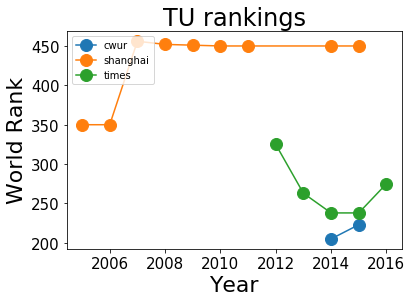
\includegraphics[width=0.45\linewidth]{graphs/tu_univie_rank_graph}
	
\end{figure}
\begin{figure}
	\centering
	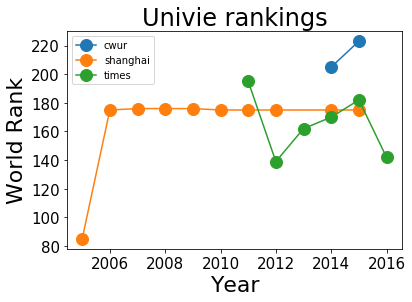
\includegraphics[width=0.45\linewidth]{graphs/tu_rank_graph}
	
\end{figure}



\end{frame}

%Ajay
\begin{frame}
\frametitle{Data exploration - Heatmap for overview}
\begin{figure}[h]
	\centering
	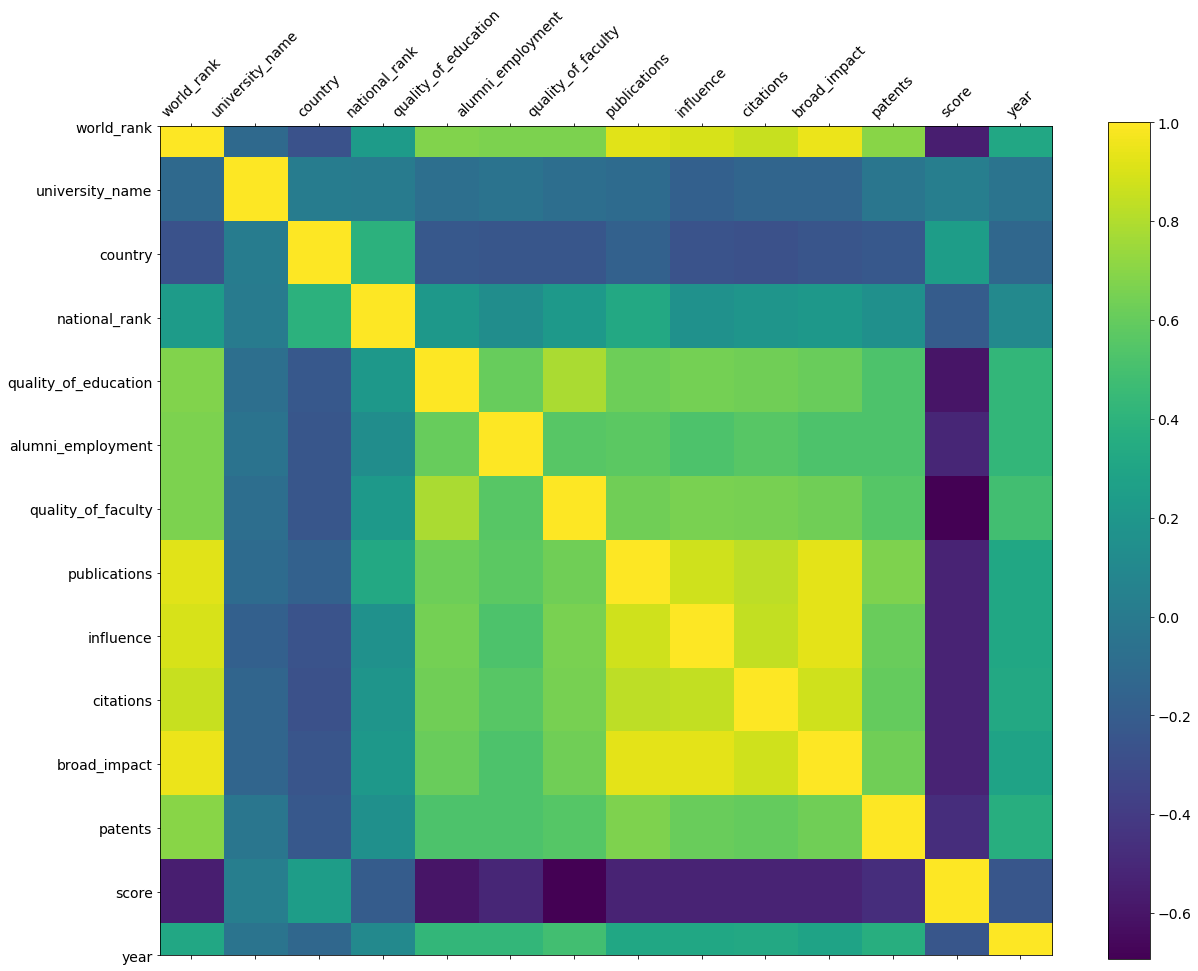
\includegraphics[width=8cm,height=8cm,keepaspectratio]{graphs/world_uni_hm}

\end{figure}

\end{frame}

%Ajay
\begin{frame}
\frametitle{Data exploration - World rank vs  other characteristics}
\begin{figure}
	\centering
	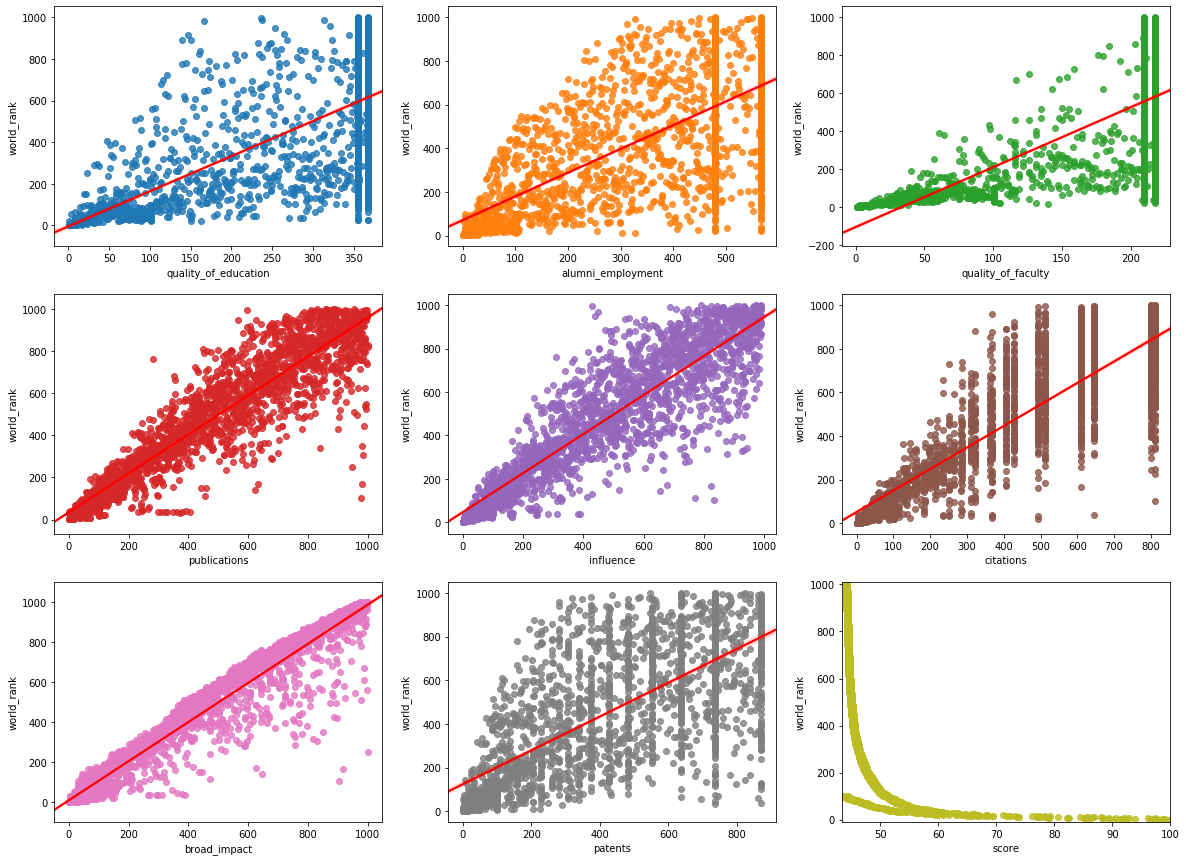
\includegraphics[width=0.9\linewidth]{graphs/rank_scatterplot}
\end{figure}

\end{frame}

\begin{frame}
\frametitle{Data exploration - Ranking by region}
\begin{figure}
	\centering
	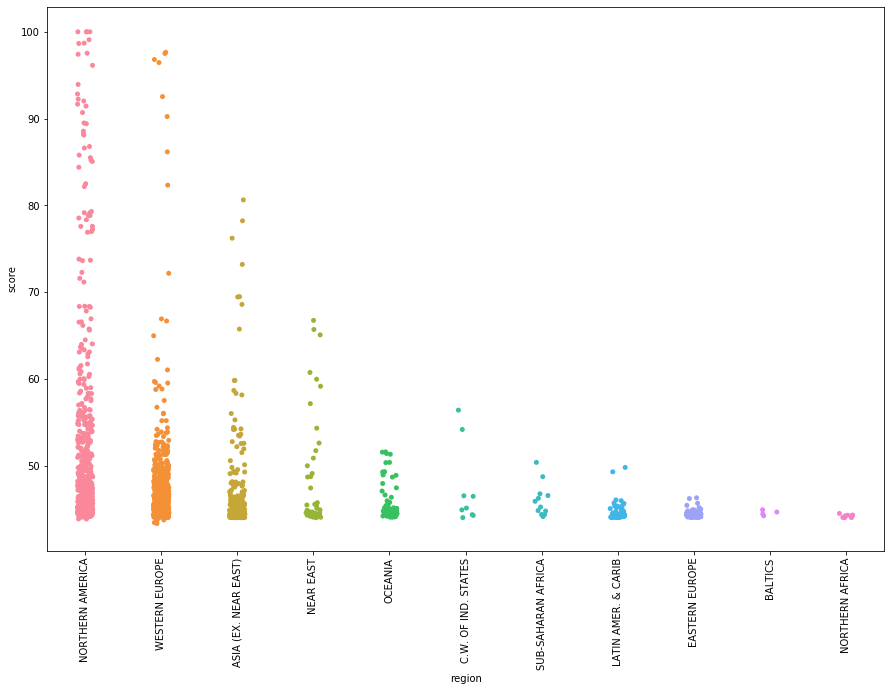
\includegraphics[width=0.9\linewidth]{graphs/region_stripplot}

\end{figure}
\end{frame}

%Julian
\begin{frame}
\frametitle{Data exploration - Ranking deviation over years (2012-2015)}
\begin{figure}
	\centering
	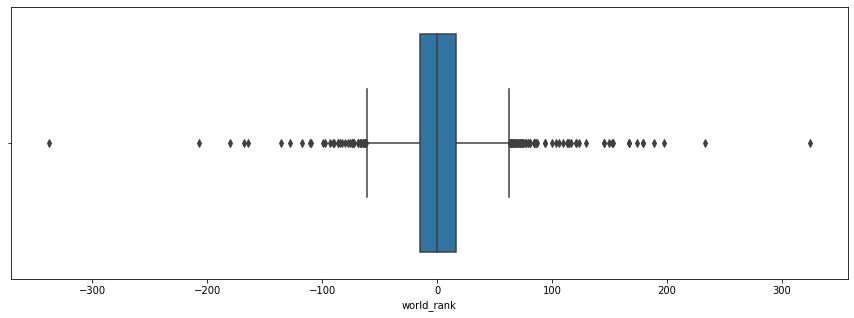
\includegraphics[width=1\linewidth]{graphs/world_rank_diff_bp}
\end{figure}
\end{frame}


%Julian
\begin{frame}
\frametitle{Data exploration - Expenditure for education}
\begin{figure}
	\centering
	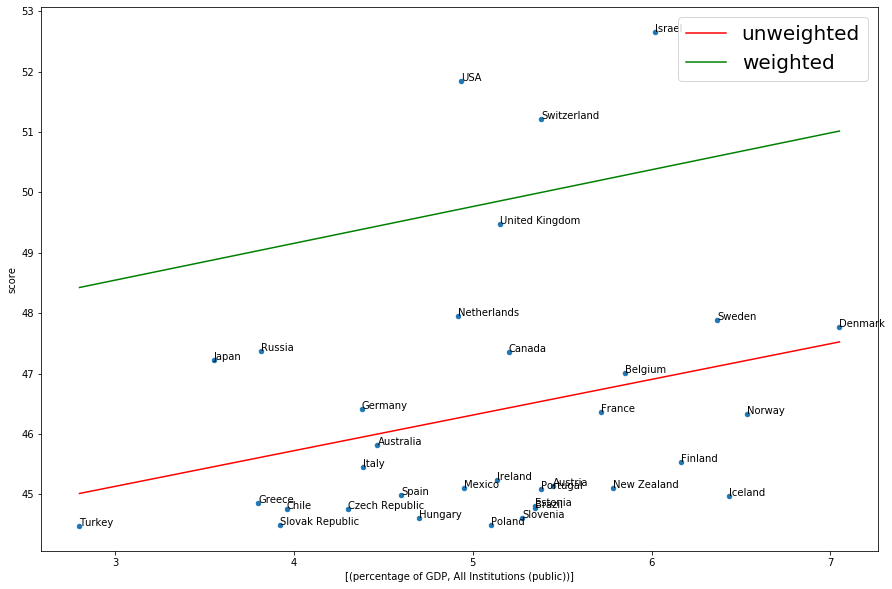
\includegraphics[width=1\linewidth]{graphs/exp_mean_all}
\end{figure}

\end{frame}

%Julian
\begin{frame}
\frametitle{Data exploration - Other results}
\begin{tabular}{|c|c|c|} \hline
\textbf{independent variable} & \textbf{dependent variable} & \textbf{impact} \\ \hline
\makecell{expenditures for education \\ (all institutions)} & mean score of country & YES \\ \hline
\makecell{expenditures for education \\ (all institutions)} & max. score of country & NO \\ \hline
\makecell{expenditures for education \\ (higher institutions)} & mean score of country & YES \\ \hline
\makecell{expenditures for education \\ (higher institutions)} & max. score of country & NO \\ \hline
\makecell{number of universities} & mean score of country & SLIGHT \\ \hline
\makecell{number of inhabitants} & mean score of country & NO \\ \hline
\makecell{univerisites per inhabitant} & mean score of country & YES \\ \hline
\makecell{HDI} & mean score of country & YES \\ \hline
\makecell{corruption} & mean score of country & NO \\ \hline

\end{tabular}

\end{frame}




%Tobi
\begin{frame} 
\frametitle{Predicting times-score}

\begin{enumerate}
\item \textbf{Setup:}

\begin{enumerate}
\item only top 200 universities from times-survey considered
\item predict times-score using number of students, student-staff-ratio, percentage of international students and percentage of female students.
\item grid-search over different ML-algorithm and parameters
\end{enumerate}

\item best ML-algorithm: random forest

\item Mean squared error: 3.4
\end{enumerate}

\end{frame}

%Tobi
\begin{frame}
\frametitle{Actual scores vs predicted scores}
\begin{figure}
\centering
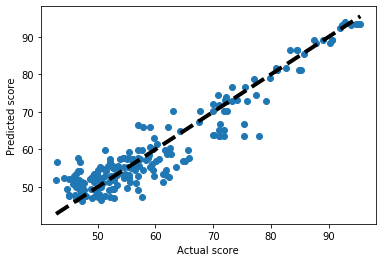
\includegraphics[width=1\linewidth]{graphs/pred_uniFeatures_unirank}
\end{figure}

\end{frame}

%Ajay
\begin{frame} 
\frametitle{Final thoughts}
\begin{itemize}

\item Working with messy data can be pretty tedious

\item Preprocessing takes up a big chunk of human and computational effort

\item Preprocessing and data cleaning essential for meaningful results

\item Acquisition of suitable data is difficult



\end{itemize}


\end{frame}

%Ajay
\begin{frame}

\centering\Huge {Thank you for your attention!}\\
\centering\Large{Any Questions?}


\end{frame}



\end{document}